\section{Линейная регрессия}

Предыдущий подход часто называют эконометрическим: он учитывает такие присущие товарам свойства как тренд и сезонность, используя статистические методы. Сейчас попробуем дать предсказание, используя базовый численный метод --- линейную регрессию.

Напомним, что модель линейной регрессии представляет собой один нейрон с $n$ входами (признаками) $x \in \setR^n$, некоторой активационной функцией и одним выходом:
$$
\hat y = f(w_0 + \langle x,\,w\rangle),
$$
где $w_0 \in \setR$, $w \in \setR^n$ --- параметры модели (веса), подбираемые методом градиентного спуска, минимизируещего некоторый функционал цены.

Мы возьмем в качестве признаком данные за 28 дней перед предсказанием и день недели. (День недели кодируется в виде семи признаков, принимающих единичное значение, если предсказывается данный день недели, иначе ноль. Такой способ кодирования позволяет задать различные веса дня каждого дня недели и не дает какому-либо дню недели априорного преимущества перед другими.) Активационную функцию возьмем линейную $f(z) = z$. Будем минимизировать средне-квадратичную ошибку $J = \frac{1}{N}\sum_{k=1}^{N} (y^k - \hat y^k)^2$, где $N$ --- размер обучающей выборки.
Обучение произведем на первых 11 месяцах.

Наша надежда в том, что, имея данные о 28 днях и о дне недели, модель сможет распознать оба вида сезонности: месячную и недельную, при этом тренд должен быть распознан за счет большого количества весов, больших единицы. В случае, когда мы хотим предсказывать данные на больший срок, чем один день, мы можем использовать значение, сгенерированное на предыдущих итерациях как признак: таким образом работают наибольшее число реккурентных моделей. Использование всего одного нейрона должно уберечь нас от переобучения модели.

На графике Рис.~\ref{img:fit} можно посмотреть качество приближения на обучающей выборке. На графике Рис.~\ref{img:test} можно посмотреть качество предсказания на проверочной выборке (декабрь). Средняя ошибка в декабре составила $64\,334,\!37$.

\begin{figure}[h]
        \noindent\centering{
        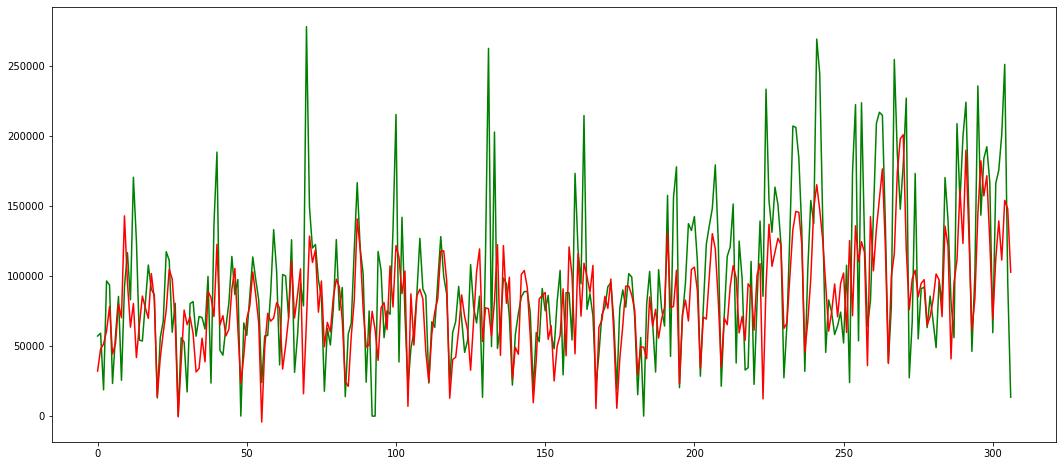
\includegraphics[width=160mm]{content/linear/fit.png}
        }
        \caption{Предсказание модели на обучающей выборке. Здесь красным --- предсказание, зеленым --- истинное значение.}
        \label{img:fit}
\end{figure}

\begin{figure}[h]
        \noindent\centering{
        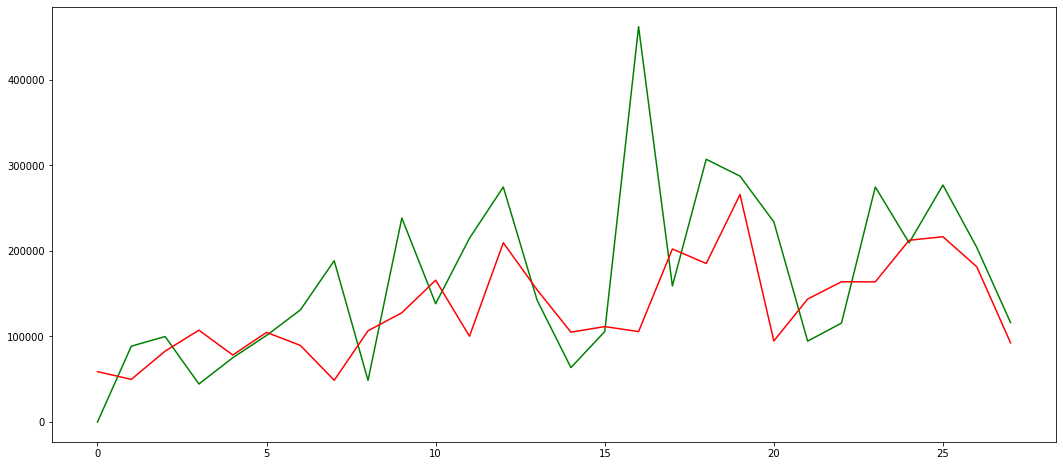
\includegraphics[width=160mm]{content/linear/test.png}
        }
        \caption{Предсказание модели на проверочной выборке (за декабрь). Здесь красным --- предсказание, зеленым --- истинное значение.}
        \label{img:test}
\end{figure}